% Main-text body.  Five-page limit: the figure, five tables, five displayed
% equations, the abstract and nineteen headings cost ~3 pages, so the prose
% budget is ~2,010 words.  Detail lives in the appendix, which does not count.
% Check with:  ../.venv/Scripts/python.exe tools/prosecount.py
%             ../.venv/Scripts/python.exe tools/pagecheck.py

\maketitle

\begin{abstract}
A design campaign accepts every sample inside a tolerance band around a target, and we
study what limits that fraction under inference-time guidance. On QM9 3D coordinates we
train an E(3)-equivariant flow-matching model against a matched diffusion baseline, and
confirm guidance works, roughly doubling coverage while molecule stability falls from
$0.434$ to between $0.199$ and $0.320$. The property error splits into centring and
spread, and one strength dial moves both. Batch-Dispersion Guidance measures the batch
spread of the guide's endpoint prediction, forms a scale-free error against a requested
setpoint, and servoes the guidance term's deviation gain by it while holding the
centring gain fixed, at no additional network evaluations. The setpoint moved the
guide-scored spread monotonically on three of three q50 curves, from $0.67$ to $1.19$
times unguided, including widening, which the strength dial does not reach.
Coverage does not improve over a tuned plug-in baseline, and over 72 paired tests the
largest effect is a loss: the coefficient is affine in the predicted property, so the
rule is the plug-in field reweighted. Transferred unchanged to DNA enhancers on the
probability simplex, the ordering reproduces and the widening does not clear noise. The
setpoint orders spread at no extra sampling cost; it is not a value the sampler attains.
\end{abstract}

\section{Introduction}

Diffusion reverses a stochastic corruption \citep{karras2022elucidating} and flow
matching regresses a vector field along a prescribed path \citep{lipman2022flow};
stochastic interpolants contain both \citep{albergo2025stochastic}, so the backbone
choice is empirical.

At a median target our batches sit $0.6$ to $3.0$ tolerance-band widths off target while
their spread is $6.0$ to $16.4$ band widths, so clustering limits coverage. Guidance
rules carry one strength dial that
moves centring and spread together \citep{ho2022classifier,zheng2023guided}, and we
found none letting the user request a spread in property units.

We test on two state spaces whether requesting batch dispersion raises band coverage:
QM9 3D coordinates, and DNA enhancers on the probability simplex. We expected the knob
to raise coverage and to transfer; it transferred and the coverage gain did not appear.
Our contributions are summarized as follows.
\begin{itemize}[leftmargin=1.1em,itemsep=0pt,topsep=1pt,parsep=0pt]
  \item We benchmark flow matching against published diffusion on one budget.
  \item We price guidance against a matched unguided control.
  \item BDG servoes the deviation gain by the batch variance of the guide's own
    endpoint prediction, at no extra network evaluations, and we state the reduction
    bounding it.
  \item The controller transfers to the simplex, where we measure the same signatures.
\end{itemize}

\section{Related Work}

\textbf{Continuous models and guidance.} Flow matching \citep{lipman2022flow},
rectified flow \citep{liu2022flow} and EDM \citep{karras2022elucidating} are endpoints
of one construction \citep{albergo2025stochastic,ma2024sit}. Our comparators are
DPS \citep{chung2023dps}, LGD-MC \citep{song2023lgd}, TMPD \citep{boys2024tmpd}, TFG
\citep{ye2024tfg} and D-Flow \citep{benhamu2024dflow}.

\textbf{Near our mechanism.} Prior work drives ensemble moments to a target
\citep{mgd2026moment}, tilts ensemble variance toward wider batches
\citep{vtd2026variance}, sets ensemble spread by the step count
\citep{ensemblevar2025}, couples trajectories
repulsively \citep{corso2024particle}, widens through negative guidance
\citep{ventura2026negative}, and reads the guidance scale as a control gain
\citep{cfgctrl2026,fbg2025feedback}. In a search we do not claim is exhaustive we did
not find a weight set by the batch variance of a \emph{learned predictor's} endpoint
prediction against a \emph{two-sided user-chosen} setpoint.

\textbf{The two modalities.} EDM defines the stability conventions we adopt
\citep{hoogeboom2022equivariant}, and property-conditioned 3D generation is our task
\citep{bao2023eegsde,xu2022geodiff,irwin2024semlaflow,song2023equifm}. On the simplex,
Dirichlet \citep{stark2024dirichlet}, Fisher \citep{davis2024fisher} flow matching and
MOG-DFM \citep{chen2025mogdfm} score the task by Fr\'echet biological distance at 500
base pairs; Gumbel-Softmax flow matching \citep{tang2025gumbel} works the simplex on
other tasks. We score GC-band coverage at 200 base pairs (Appendix~A.4).

\section{Methods}

\subsection{Modalities, Data, and Preprocessing}
\label{sec:data}

\textbf{Modality 1} is QM9, 133{,}885 molecules on $\mathbb{R}^{N\times3}$: coordinates
zero-centred, a hard one-hot over $\{$H,C,N,O,F$\}$, no feature scaling. Splits are \texttt{train\_a} for the generator and guide $f_A$,
\texttt{train\_b} for the evaluator $f_B$, and \texttt{val} and \texttt{test} held out
(Appendix~A.1). We generate unconditionally; the properties are dipole
$\mu$ (D), polarizability $\alpha$ (Bohr$^3$) and HOMO-LUMO gap (Ha).

\textbf{Modality 2} is 6{,}126 \emph{Drosophila} Kenyon-cell enhancer regions
\citep{chen2025mogdfm} on $(\Delta^3)^L$ at $L{=}200$, decoded by per-position
$\arg\max$: no rotation group, and an exact property.

\subsection{Continuous Flow Matching Baseline}
\label{sec:fm}

With $t:0\to1$ from noise to data, the linear interpolant $x_t = t x_1 + (1-t) x_0$ has
constant conditional velocity $u_t=x_1-x_0$, and the source is projected onto the
zero-centre-of-mass subspace of dimension $3(N-1)$. The objective is a masked mean over
$t\sim\mathcal{U}(0,1)$, coordinates and types normalised separately, $\lambda=1$:
\begin{equation}
\mathcal{L}_{\mathrm{FM}}(\theta)=
\mathbb{E}_{t,x_0,x_1}\!\left[
\tfrac{1}{3\Sigma M}\big\|M\odot(v^{c}_\theta - u^{c})\big\|^2
+\lambda\tfrac{1}{K\Sigma M}\big\|M\odot(v^{f}_\theta - u^{f})\big\|^2
\right],
\label{eq:fmloss}
\end{equation}
with $M$ the atom mask, $\Sigma M$ its sum, $K$ the type channels and the superscripts
$c$, $f$ the coordinate and type heads. The network is a dense E(3)-equivariant graph
network of 3.75\,M parameters; Table~\ref{tab:a-train} gives its architecture and
optimiser settings. We sample with explicit Euler in 100 steps.

\subsection{Diffusion Baseline}
\label{sec:diff}

The diffusion baseline shares everything with Section~\ref{sec:fm} but the corruption,
which makes Section~\ref{sec:fmvd} interpretable: a variance-preserving process with
$\beta(\tau)=\beta_{\min}+\tau(\beta_{\max}-\beta_{\min})$, $\beta_{\min}=0.1$,
$\beta_{\max}=20$:
\begin{equation}
x_\tau=\alpha(\tau)x_0+\sigma(\tau)\epsilon,
\quad
\log\alpha(\tau)=-\tfrac12\big(\beta_{\min}\tau+\tfrac12(\beta_{\max}-\beta_{\min})\tau^2\big),
\quad \alpha^2+\sigma^2=1 .
\label{eq:vp}
\end{equation}
The network predicts $\epsilon$. We integrate
$\mathrm{d}x/\mathrm{d}\tau=-\tfrac12\beta(\tau)(x+s_\theta)$ backwards,
$s_\theta=-\epsilon_\theta/\sigma$, on a decreasing 100-step grid, then jump to the
Tweedie mean.

\subsection{Guided Generation}
\label{sec:guidance}

Each guided step toward target $y$ forms the endpoint estimate $m_i$, being
$x_t^{(i)}+(1-t)v_\theta(x_t^{(i)},t)$ for the flow model and the Tweedie mean for the
diffusion model, evaluates $F_i=f_A(m_i)$ and $g_i=\nabla_m f_A(m_i)$, and adds
\begin{equation}
G_i \;=\; \frac{\mathrm{num}_i}{s^2}\,J_i^{\!\top} g_i ,
\qquad
\mathrm{num}_i^{\mathrm{plug}} \;=\; y - F_i ,
\label{eq:plug}
\end{equation}
where $J_i$ is the Jacobian of the endpoint map $x_t\!\mapsto\!m_i$ and $s$ is the
guide's target standard deviation. The
sampler scales it by $w(1-t)/t$ and clips to a velocity-relative trust region, without
which a pilot diverged $222$ of $3{,}328$ samples. Guidance runs for
$t\ge0.5$, a $50$-step window, on batches of $B=256$.

\subsection{Proposed Innovation: Batch-Dispersion Guidance}
\label{sec:bdg}

\textbf{Mechanism.} For a batch BDG forms the mean $\Fbar$, the unbiased variance $\Vb$
and the scale-free error $e=(\Vb-\tau^2)/\tau^2$ against a setpoint $\tau$, then
replaces the numerator of Equation~\eqref{eq:plug} by
\begin{equation}
\mathrm{num}_i \;=\; (y-F_i)\;-\;\eta\,e\,\big(F_i-\Fbar\big)
\;=\;\big(y-\Fbar\big)-\weff\big(F_i-\Fbar\big),
\qquad \weff=1+\eta e .
\label{eq:bdgnum}
\end{equation}
$\Vb>\tau^2$ contracts the batch and $\Vb<\tau^2$ expands it; both terms multiply the
same $g_i$. Algorithm~\ref{alg:bdg} is the whole step
and Figure~\ref{fig:mechanism} is it measured.

\textbf{The reduction.} Equation~\eqref{eq:bdgnum} is affine in $F_i$, so it factors
exactly,
\begin{equation}
(y-F_i)-\eta e\big(F_i-\Fbar\big)=\big(1+\eta e\big)\big(y_{\mathrm{eff}}-F_i\big),
\qquad
y_{\mathrm{eff}}=\frac{y+\eta e\,\Fbar}{1+\eta e},
\label{eq:reduction}
\end{equation}
making BDG the plug-in field at a rescaled weight and a shifted target. The reduction
constrains the step and not the method, since no fixed weight reproduces a gain that
changes sign online.

\textbf{Properties and controls.} Since $\Vb\ge0$, $\weff\ge1-\eta$ for any batch,
licensing two-sided operation and forcing $\eta>1$. The equilibrium
$V^{\star}=\tau^2(1-1/\eta)$ is an asymptote the window does not reach. Two settings
are \emph{gates}: $\eta=0$ and the
one-sided variant must each reproduce the plug-in field exactly. Three controls isolate
the mechanism: a strength sweep at fixed $(\eta,\tau)$, an open-loop replay of a
recorded $e$ schedule on another seed, and a matched signed-$w$ plug-in control, which
our drop rule turns on: if it reaches BDG's spread at equal chemistry, we withdraw the
claim.

\subsection{Transfer to Modality 2}
\label{sec:transfer}

BDG's step is a per-sample scalar times the plug-in step, so no inverse is required
where $\mathrm{diag}(p)-pp^\top$ is singular. The state space, generator
and property map change; GC content relaxes analytically and its exact count is the
evaluator. The $t\ge0.5$ window carries over unchanged, where GC batch spread is nearly
flat. Appendix~A.2 gives the Modality 2 architecture, training and this window's cost.

\subsection{Model Overview}
\label{sec:overview}

Figure~\ref{fig:overview} sets out the study.

\begin{figure}[!tb]
  \centering
  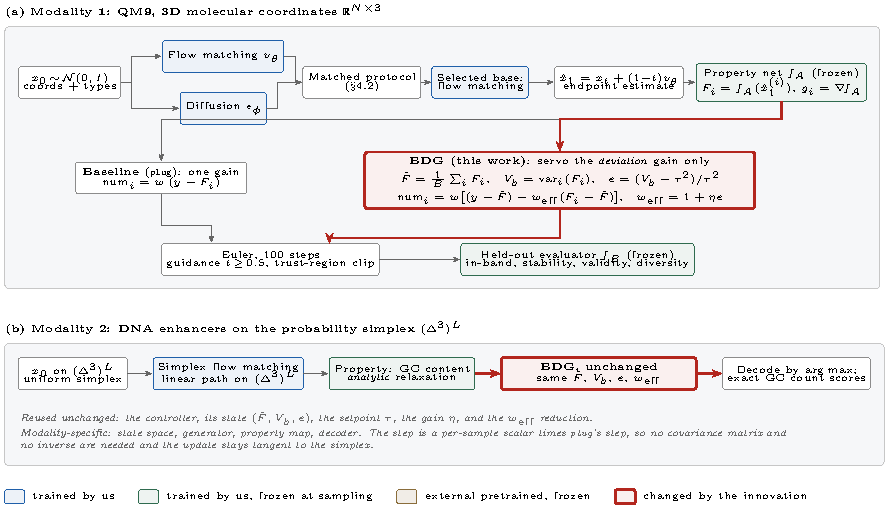
\includegraphics[width=0.52\linewidth]{figs/overview.pdf}
  \caption{Study overview. \textbf{(a)} one representation feeds a flow-matching and a
  diffusion model; the plug-in baseline applies one gain to $(y-F_i)$, BDG holds the
  centring gain at $w$ and servoes only $\weff$. \textbf{(b)} the same controller on the
  simplex. Blue trained here, grey frozen, tan pretrained, red changed by BDG.}
  \label{fig:overview}
\end{figure}

\section{Results}

\subsection{Evaluation Protocol}
\label{sec:protocol}

The target metric is \ib, the fraction of molecules whose property, scored by the
held-out $f_B$, falls within $\pm\delta$ of the target, $\delta$ being twice the
evaluator's calibration mean absolute error. We report
\ib{} on decoded molecules and the spread ratio against unguided, at the \textbf{q50}
target, the median of the training property distribution. The \emph{chemistry floor} is
$0.9\times$ the unguided arm's molecule stability, and we do not rank an arm below it.
Arms
share the checkpoint, guide, evaluator, target, atom counts and noise, and
Table~\ref{tab:guidance} reports each arm's best strength.
Spread ratios are scored by $f_A$ and \ib{} by the held-out $f_B$.
Table~\ref{tab:fmvd} uses three seeds; every other cell uses one at $n{=}256$, where the
standard error on \ib{} is about $0.02$.

\subsection{Modality 1: Flow Matching versus Diffusion}
\label{sec:fmvd}

\begin{table}[!tb]
\centering\tiny
\setlength{\tabcolsep}{4pt}
\caption{Base models on QM9, unconditional, 100-step Euler ODE, our evaluator under EDM
conventions. Our flow row is three seeds of 10{,}000 samples, $\pm$ one seed sd;
\texttt{EDMsecond} is borrowed, $n{=}2{,}000$, one seed, so it is not comparable.
\pend{} is pending (Appendix~A.7).}
\label{tab:fmvd}
\begin{tabular}{llrrrrrr}
\toprule
Model & Source & Atom stab.$\uparrow$ & Mol.\ stab.$\uparrow$ & Validity$\uparrow$ & Uniq.$\uparrow$ & NFE$\downarrow$ & Params \\
\midrule
Flow matching (ours)          & reproduced & $0.9366${\tiny$\pm.0012$} & $0.3993${\tiny$\pm.0085$} & $0.7625${\tiny$\pm.0031$} & $0.9939$ &  $100$ & $3.75$\,M \\
VP diffusion (ours)           & reproduced & \pend    & \pend    & \pend    & \pend    &  $101$ & $3.75$\,M \\
\midrule
\texttt{EDMsecond} \citep{hoogeboom2022equivariant} & borrowed & $0.9644$ & $0.6725$ & $0.8490$ & \pend & $100$ & $5.34$\,M \\
EDM \citep{hoogeboom2022equivariant} & quoted & $0.9870$ & $0.8200$ & $0.9190$ & $-$ & $1000$ & $-$ \\
Real QM9 (ceiling)            & measured   & $0.994$ & $0.956$ & $0.982$ & $-$ & $-$ & $-$ \\
\bottomrule
\end{tabular}
\end{table}

In Table~\ref{tab:fmvd} our flow model reached $0.9366$ atom and $0.3993$
molecule stability at 100 evaluations, against EDM's published $0.9870$ and $0.8200$. We
did not test the causes of that gap; EDM's own ablation of unscaled one-hot features
loses 3 atom and 35 molecule points \citep{hoogeboom2022equivariant}. We carry flow
matching forward without a fidelity win, because the diffusion row is pending, and take
the endpoint estimate from its linear path.

\subsection{Modality 1: Guidance Works}
\label{sec:guidworks}

\begin{table}[!tb]
\centering\tiny
\setlength{\tabcolsep}{4.5pt}
\caption{Guided against unguided at q50, otherwise matched. Cells are $\mu$ / gap /
$\alpha$; bold is the best guided arm in a column, a dash a cell we did not run. Every
guided arm falls below the $0.390$ chemistry floor. TFG is ported, not tuned here
(Appendix~A.4).}
\label{tab:guidance}
\begin{tabular}{lrrr}
\toprule
Arm & \ib$\uparrow$ & Spread\,/\,unguided & Mol.\ stab.$\uparrow$ \\
\midrule
unguided                  & $0.090$\,/\,$0.121$\,/\,$0.051$ & $1.00$\,/\,$1.00$\,/\,$1.00$ & $0.434$\,/\,$0.434$\,/\,$0.434$ \\
plug-in (best $w$)        & $0.184$\,/\,$0.219$\,/\,$\mathbf{0.133}$ & $0.52$\,/\,$0.60$\,/\,$0.47$ & $0.246$\,/\,$0.199$\,/\,$0.320$ \\
TFG ($w{=}4$, $\mu$ only) & $\mathbf{0.535}$\,/\,$-$\,/\,$-$ & $0.22$\,/\,$-$\,/\,$-$ & $0.172$\,/\,$-$\,/\,$-$ \\
BDG ($w{=}32$)            & $0.180$\,/\,$\mathbf{0.227}$\,/\,$0.106$ & $0.49$\,/\,$0.68$\,/\,$0.53$ & $\mathbf{0.348}$\,/\,$0.262$\,/\,$0.340$ \\
\bottomrule
\end{tabular}
\end{table}

Guidance raised \ib{} by $2.0\times$ on $\mu$, $1.8\times$ on the gap and $2.6\times$
on $\alpha$ for the plug-in rule, and TFG reached $5.9\times$ on $\mu$
(Table~\ref{tab:guidance}). TFG took the most coverage here and
the least chemistry, which is the trade-off BDG is built to make requestable.

\subsection{Modality 1: Innovation Ablations}
\label{sec:ablations}

\begin{table}[!tb]
\centering\tiny
\setlength{\tabcolsep}{4pt}
\caption{BDG ablations on $\mu$ at q50: gates, ladder, controls.
$\tau_{\mathrm{mult}}$ scales the setpoint by the unguided batch's spread, so $1.0$
requests it; rungs $0.75$ and $1.25$ and the other two properties are in
Table~\ref{tab:a-ladder}. $w{=}1$, floor $0.390$.}
\label{tab:ablation}
\begin{tabular}{llrrrrr}
\toprule
Variant & Role & $\eta$ & $\tau_{\mathrm{mult}}$ & Spread\,/\,ung. & \ib$\uparrow$ & Mol.\ stab.$\uparrow$ \\
\midrule
plug-in, $w{=}1$       & base    & $-$ & $-$   & $0.714$ & $0.1094$ & $0.3633$ \\
BDG $\eta{=}0$         & gate    & $0$ & $1.0$ & $0.714$ & $0.1094$ & $0.3633$ \\
BDG one-sided, expand  & gate    & $4$ & $1.5$ & $0.714$ & $0.1094$ & $0.3633$ \\
\midrule
BDG contract           & ladder  & $4$ & $0.5$ & $0.670$ & $0.1406$ & $0.3359$ \\
BDG neutral            & ladder  & $4$ & $1.0$ & $0.900$ & $0.0820$ & $0.4258$ \\
BDG expand             & ladder  & $4$ & $1.5$ & $1.093$ & $0.0703$ & $0.4141$ \\
\midrule
plug-in, $w{=}4$       & control & $-$ & $-$   & $0.584$ & $0.1406$ & $0.2656$ \\
open-loop $e$ replay   & control & $4$ & $0.5$ & $0.686$ & \pend    & \pend    \\
signed-$w$ plug-in     & control & $-$ & $-$   & \pend   & \pend    & \pend    \\
\bottomrule
\end{tabular}
\end{table}

The gates passed exactly in Table~\ref{tab:ablation}: at $\eta=0$ and in the one-sided
variant at an expanding setpoint, BDG reproduced the plug-in field to zero.
The setpoint moved spread monotonically on three of three q50 curves, $0.670$ to
$1.187$ times unguided (Table~\ref{tab:a-ladder}, Figure~\ref{fig:mechanism}), and the
deviation gain changed sign within a trajectory. Coverage did not improve. Every rung clearing the
chemistry floor is nominally worse than plug-in, and the largest effect over 72 paired
tests is a BDG \emph{loss} at $z=-3.07$; the grid is correlated, so we read it as a
null. Plug-in at $w=4$ reaches BDG's contraction
rung at the same \ib{}, on lower molecule stability,
a difference of $z=1.73$ that one seed does not resolve and that sits below the floor
either way; and the open-loop replay recovers 69.5\% to 96\% of the closed loop's spread
shift, so the schedule and not the feedback carries most of it.

\subsection{Modality 1: Comparison with Recent Methods}
\label{sec:recent}

\begin{table}[!tb]
\centering\tiny
\setlength{\tabcolsep}{4pt}
\caption{Four recent guidance rules ported to our frozen checkpoint, guide and evaluator
at q50, $w{=}1$. No result cell has run. Passes are network calls at batch granularity
per cell of $n{=}5{,}000$; the generator column differs across arms, so read the two
together.}
\label{tab:recent}
\begin{tabular}{llrrrrr}
\toprule
Method & Status & \ib$\uparrow$ & Mol.\ stab.$\uparrow$ & Diversity$\uparrow$ & Gen.\ passes & Guide passes \\
\midrule
DPS-style plug-in \citep{chung2023dps}  & reproduced & \pend & \pend & \pend & $10{,}000$ & $4{,}000$ \\
TMPD-inspired \citep{boys2024tmpd}      & reproduced & \pend & \pend & \pend & $10{,}000$ & $4{,}000$ \\
LGD-MC \citep{song2023lgd}              & reproduced & \pend & \pend & \pend & $12{,}000$ & $20{,}000$ \\
TFG \citep{ye2024tfg}                   & reproduced & \pend & \pend & \pend & $8{,}000$  & $20{,}000$ \\
\midrule
Flow matching, unguided                 & internal   & \pend & \pend & \pend & $10{,}000$ & $0$ \\
\textbf{BDG (ours)}                     & ours       & \pend & \pend & \pend & $10{,}000$ & $4{,}000$ \\
\bottomrule
\end{tabular}
\end{table}

We ported four guidance rules to one frozen generator (Table~\ref{tab:recent});
Appendix~A.4 gives three port caveats. BDG makes one guide forward and one backward per
guided step, the plug-in rule's exact call pattern.

\subsection{Modality 2: Transfer of the Innovation}
\label{sec:m2}

\begin{table}[!tb]
\centering\tiny
\setlength{\tabcolsep}{5pt}
\caption{Transfer to DNA enhancers on the simplex, $L{=}200$. We score GC-band coverage,
not these papers' FBD at 500 base pairs, so their numbers are never pooled with ours.}
\label{tab:m2}
\begin{tabular}{lcc}
\toprule
Signature & QM9 & DNA simplex \\
\midrule
$\eta{=}0$ reproduces plug-in & bit-identical & bit-identical \\
one-sided at an expanding setpoint & exact & exact, $\weff{=}{+}1.000$ \\
setpoint ladder monotone in spread & $0.67\!\to\!1.19$ & $0.81\!\to\!1.01$ \\
contraction breaks the chemistry floor & yes & yes \\
\ib{} improves & no & no \\
\midrule
\multicolumn{3}{l}{\emph{Against recent simplex sequence models}}\\
Dirichlet FM \citep{stark2024dirichlet} & \pend & \pend \\
Fisher Flow \citep{davis2024fisher} & \pend & \pend \\
MOG-DFM \citep{chen2025mogdfm} & \pend & \pend \\
\textbf{BDG, transferred (ours)} & \pend & \pend \\
\bottomrule
\end{tabular}
\end{table}

BDG transferred with no change to the controller and coverage did not improve
(Table~\ref{tab:m2}). The ladder's range is $1.7$ to $2.6\times$ smaller, and its
widening rung reaches only $1.006$ to $1.008$, inside the noise at this $n$, so the
ordering transfers and the widening does not. GC is affine in the simplex coordinates
and averages over 200 positions.

\subsection{Cross-Modality Analysis and Failure Modes}
\label{sec:failure}

The direction matched across modalities and the magnitude did not, which the property
map accounts for. The trust region acts at large $|\weff|$: in
Table~\ref{tab:guidance}'s cells the plug-in rule clips $701$ sample steps where BDG
clips $4{,}457$, so a rung can be clip-limited and not controller-limited. And this grid
cannot separate chemistry cost from $|\weff|$ and $\tau_{\mathrm{mult}}$.
Figure~\ref{fig:a-failures} shows what contraction breaks.

\section{Discussion}

Guidance worked at a measured chemistry cost, and the ablations support one mechanism
claim beside one null on coverage. Both transferred to the simplex.

Equation~\eqref{eq:reduction} accounts for the null. BDG reaches nothing outside the
plug-in field's two-parameter family, and we swept one of those parameters. The one
chemistry gain we measure, $+0.07$ at $n{=}256$, is unresolved at $z=1.73$.

Four limitations bound the claim: the trust region confounds the largest rungs, the
signed-$w$ control has not run, the open-loop control rests on one seed pair, and both
cells of the chemistry comparison sit below our floor. The narrowest claim supported is monotone, two-sided,
modality-portable spread control at no extra sampling cost, the setpoint ordering spread
without attaining it.
